\chapter{Contexte du stage}
\label{AnalyseConception}

\section{Environnement de travail}

Durant le stage j'ai travaillé sur un pc de marque Dell, dont le système d'exploitation est Windows 8.1 Profesionnal (machine hôte). L'entreprise travaille avec de nombreuses machines virtuelles hébergées ou distantes afin de disposer d'environnement de tests, de développements, et de production. Pour cela, j'avais à ma disposition une machine virtuelle de développement via VirtualBox avec le système d'exploitation Windows Server 2012 R2 Standard. \\

\section{Outils utilisés}

Quotidiennement j'ai utilisé 2 environnements de développement intégré (IDE) : Liclipse (pour développer en langage Python) dans le projet DataWizard, et \textbf{Eclipse} version Mars (pour développer en langage Java/Java EE) pour les projets MobiSaaS et Crislab.\\

J'ai manipulé plusieurs \textbf{SGBD} : MongoDB (MobiSaaS), Oracle (Crislab), mais j'ai principalement travaillé avec le couple \textbf{Postgresql}/\textbf{Postgis} afin de gérer les données géographiques dans les 2 projets "DataWizard" \& "MobiSaaS".\\

Afin de tester les web services REST développés, j'ai utilisé fréquemment l'outil \textbf{SoapUI} (Fig. \ref{SoapUIGet}). Il permet de mettre en place une suite de tests qui peuvent être lancé d'une traite du côté client, permet de tester les services web en mode bouchon mais aussi d'effectuer des tests de charge. Il permet entre autre de fournir une hiérarchie des services web, de lister les différentes méthodes disponible, les paramètres attendus, de réaliser des requêtes et de récupérer les réponses … C'est l'un des meilleurs outils de test unitaires concernant les services web.

\begin{center}
\begin{figure}[h] \centering
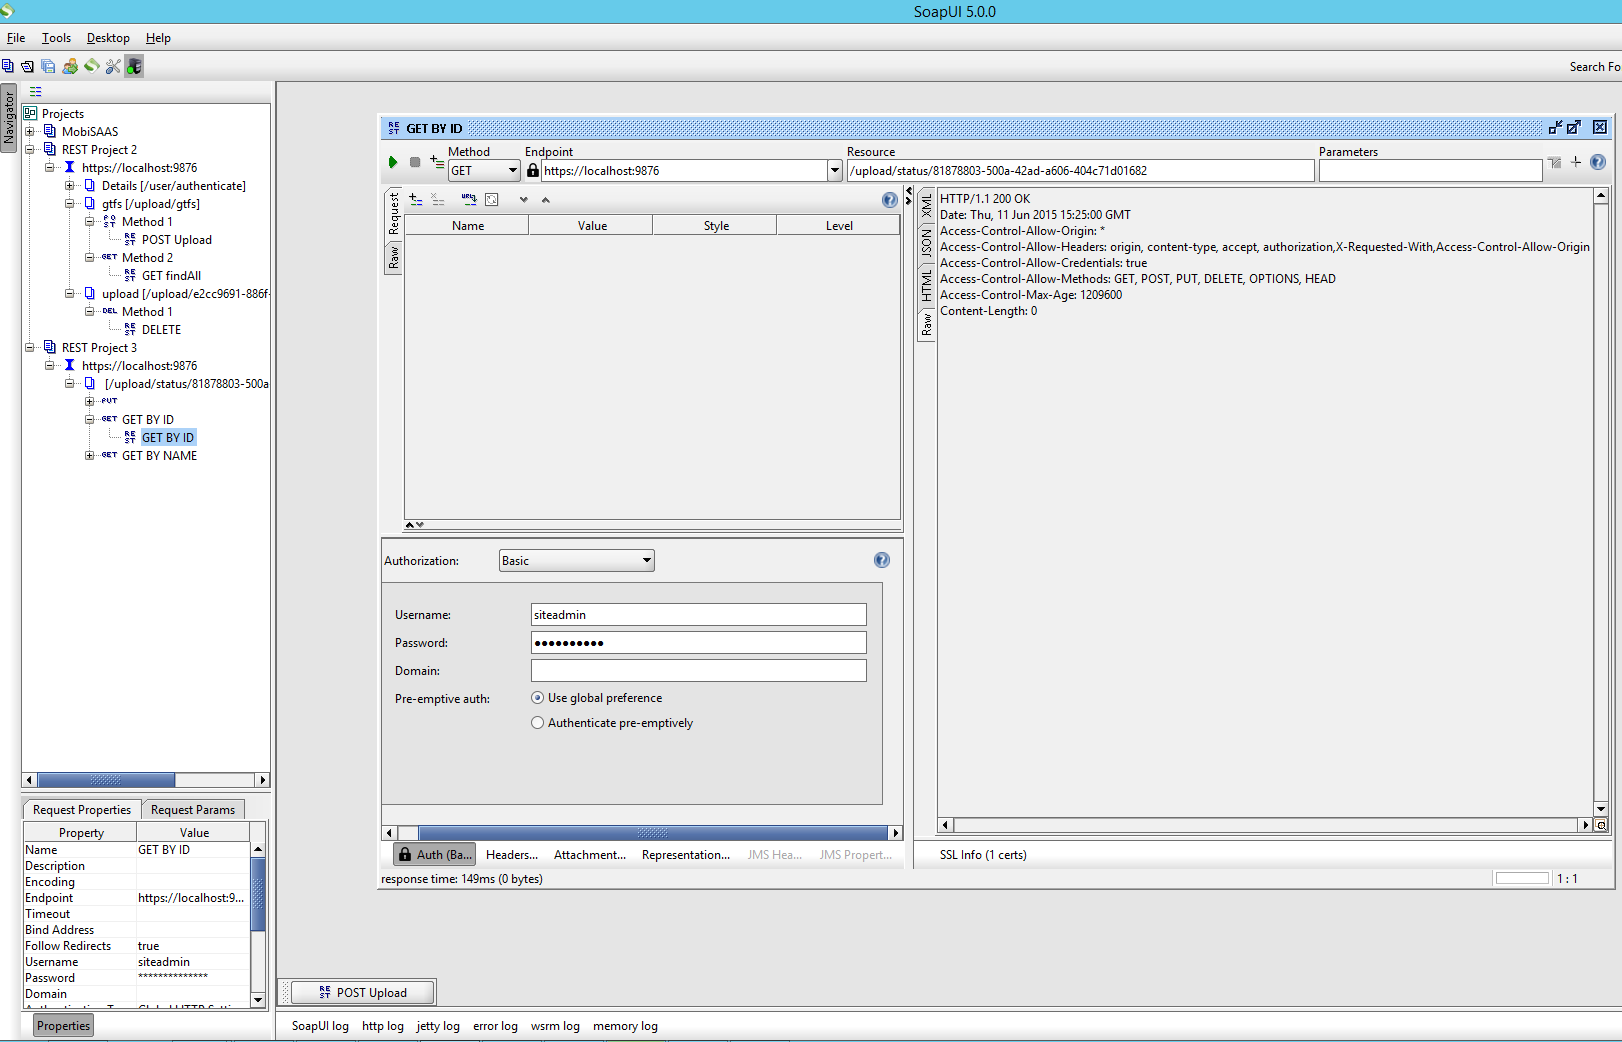
\includegraphics[width=16cm]{images/soapUI_getById_sansResponse_small.png}\\
\caption{\label{SoapUIGet} Interface et exemple de requête "GET" SoapUI}
\end{figure}
\end{center}


\section{Gestion de projets}

Dans les projets auxquels j'ai participé, l'entreprise utilise des outils de gestion : planning, suivi de bugs, outils de mutualisation, gestion de versions. Ainsi, j'ai utilisé l'outil Trello pour la gestion des tâches, Redmine pour la gestion des projets (cf. Annexe \ref{Annexe C}), et \textbf{SVN} pour la gestion des codes sources. L'entreprise met à disposition de ses salariés un intranet avec de nombreux outils collaboratifs sous la plateforme eGroupware (Feuille de temps,etc...).\\

Un point de suivi informel était effectué plusieurs fois par semaine avec l'encadrant afin de présenter le travail effectué, les résultats intermédiaires, et le travail planifié pour la semaine suivante. Un bilan à la mi-stage a été effectué afin de réajuster les priorités, et arriver à produire un livrable satisfaisant en fin de stage. De plus, de nombreuses tâches de soutien aux équipes arrivaient au fil de l'eau : productions de réseaux de transport, tests, etc...\\

